\PassOptionsToPackage{unicode=true}{hyperref} % options for packages loaded elsewhere
\PassOptionsToPackage{hyphens}{url}
\documentclass[11pt,dvipsnames,ignorenonframetext,aspectratio=169]{beamer}
\IfFileExists{pgfpages.sty}{\usepackage{pgfpages}}{}
\setbeamertemplate{caption}[numbered]
\setbeamertemplate{caption label separator}{: }
\setbeamercolor{caption name}{fg=normal text.fg}
\beamertemplatenavigationsymbolsempty
\usepackage{lmodern}
\usepackage{amssymb,amsmath}
\usepackage{ifxetex,ifluatex}
\usepackage{fixltx2e} % provides \textsubscript
\ifnum 0\ifxetex 1\fi\ifluatex 1\fi=0 % if pdftex
  \usepackage[T1]{fontenc}
  \usepackage[utf8]{inputenc}
\else % if luatex or xelatex
  \ifxetex
    \usepackage{mathspec}
  \else
    \usepackage{fontspec}
\fi
\defaultfontfeatures{Ligatures=TeX,Scale=MatchLowercase}







\fi

  \usetheme[]{monash}

  \usecolortheme{monashwhite}


% A default size of 24 is set in beamerthememonash.sty


  \useinnertheme{rounded}

  \useoutertheme{smoothtree}

% use upquote if available, for straight quotes in verbatim environments
\IfFileExists{upquote.sty}{\usepackage{upquote}}{}
% use microtype if available
\IfFileExists{microtype.sty}{%
  \usepackage{microtype}
  \UseMicrotypeSet[protrusion]{basicmath} % disable protrusion for tt fonts
}{}


\newif\ifbibliography


\hypersetup{
      pdftitle={Developmental genetics},
            colorlinks=true,
    linkcolor=red,
    citecolor=Blue,
    urlcolor=lightgrayd,
    breaklinks=true}
%\urlstyle{same}  % Use monospace font for urls







% Prevent slide breaks in the middle of a paragraph:
\widowpenalties 1 10000
\raggedbottom

  \AtBeginPart{
    \let\insertpartnumber\relax
    \let\partname\relax
    \frame{\partpage}
  }
  \AtBeginSection{
    \ifbibliography
    \else
      \let\insertsectionnumber\relax
      \let\sectionname\relax
      \frame{\sectionpage}
    \fi
  }
  \AtBeginSubsection{
    \let\insertsubsectionnumber\relax
    \let\subsectionname\relax
    \frame{\subsectionpage}
  }



\setlength{\parindent}{0pt}
\setlength{\parskip}{6pt plus 2pt minus 1pt}
\setlength{\emergencystretch}{3em}  % prevent overfull lines
\providecommand{\tightlist}{%
  \setlength{\itemsep}{0pt}\setlength{\parskip}{0pt}}

  \setcounter{secnumdepth}{0}


%% Monash overrides
\AtBeginSection[]{
   \frame<beamer>{
   \frametitle{Outline}\vspace*{0.2cm}
   
   \tableofcontents[currentsection,hideallsubsections]
  }}

% Redefine shaded environment if it exists (to ensure text is black)
\ifcsname Shaded\endcsname
  \definecolor{shadecolor}{RGB}{225,225,225}
  \renewenvironment{Shaded}{\color{black}\begin{snugshade}\color{black}}{\end{snugshade}}
\fi
%%

  \usepackage{setspace}
  \usepackage{wasysym}
  % \usepackage{footnote} % don't use this this breaks all
  \usepackage{fontenc}
  \usepackage{fontawesome}
  \usepackage{booktabs,siunitx}
  \usepackage{longtable}
  \usepackage{array}
  \usepackage{multirow}
  \usepackage{wrapfig}
  \usepackage{float}
  \usepackage{colortbl}
  \usepackage{pdflscape}
  \usepackage{tabu}
  \usepackage{threeparttable}
  \usepackage{threeparttablex}
  \usepackage[normalem]{ulem}
  \usepackage{makecell}
  \usepackage{xcolor}
  \usepackage{tikz} % required for image opacity change
  \usepackage[absolute,overlay]{textpos} % for text formatting
  \usepackage{chemfig}
  \usepackage[skip=0.333\baselineskip]{caption}
  % \newcommand*{\AlignChar}[1]{\makebox[1ex][c]{\ensuremath{\scriptstyle#1}}}%
  
  % this font option is amenable for beamer
  \setbeamerfont{caption}{size=\tiny}
  \singlespacing
  \definecolor{lightgrayd}{gray}{0.95}
  \definecolor{skyblued}{rgb}{0.65, 0.6, 0.94}
  \definecolor{oranged}{RGB}{245, 145, 200}

  \title[]{Developmental genetics}


  \author[
        Deependra Dhakal\\
Gokuleshwor Agriculture and Animal Science College\\
Tribhuwan University\\
\textit{ddhakal.rookie@gmail.com}\\
\url{https://rookie.rbind.io}
    ]{Deependra Dhakal\\
Gokuleshwor Agriculture and Animal Science College\\
Tribhuwan University\\
\textit{ddhakal.rookie@gmail.com}\\
\url{https://rookie.rbind.io}}


\date[
      Academic year 2019-2020
  ]{
      Academic year 2019-2020
        }

\begin{document}

% Hide progress bar and footline on titlepage
  \begin{frame}[plain]
  \titlepage
  \end{frame}


   \frame<beamer>{
   \frametitle{Outline}\vspace*{0.2cm}
   
   \tableofcontents[hideallsubsections]
  }

\hypertarget{variegation-in-biological-tissues}{%
\section{Variegation in biological
tissues}\label{variegation-in-biological-tissues}}

\begin{frame}{Variegation: meaning}
\protect\hypertarget{variegation-meaning}{}

\begin{columns}[T,onlytextwidth]
  \small
  \column{.30\linewidth}
  
  \begin{itemize}
  \item Variegation is the appearance of differently coloured zones in the leaves, and sometimes the stems, of plants. Variegated leaves occur rarely in nature.
  \item Causes are: Chimeral, Pigmentary, Pathological (Mosaic viruses), Genetical due to transposable elements
  \end{itemize}
  
  \column{0.70\linewidth}
  
\begin{figure}

{\centering 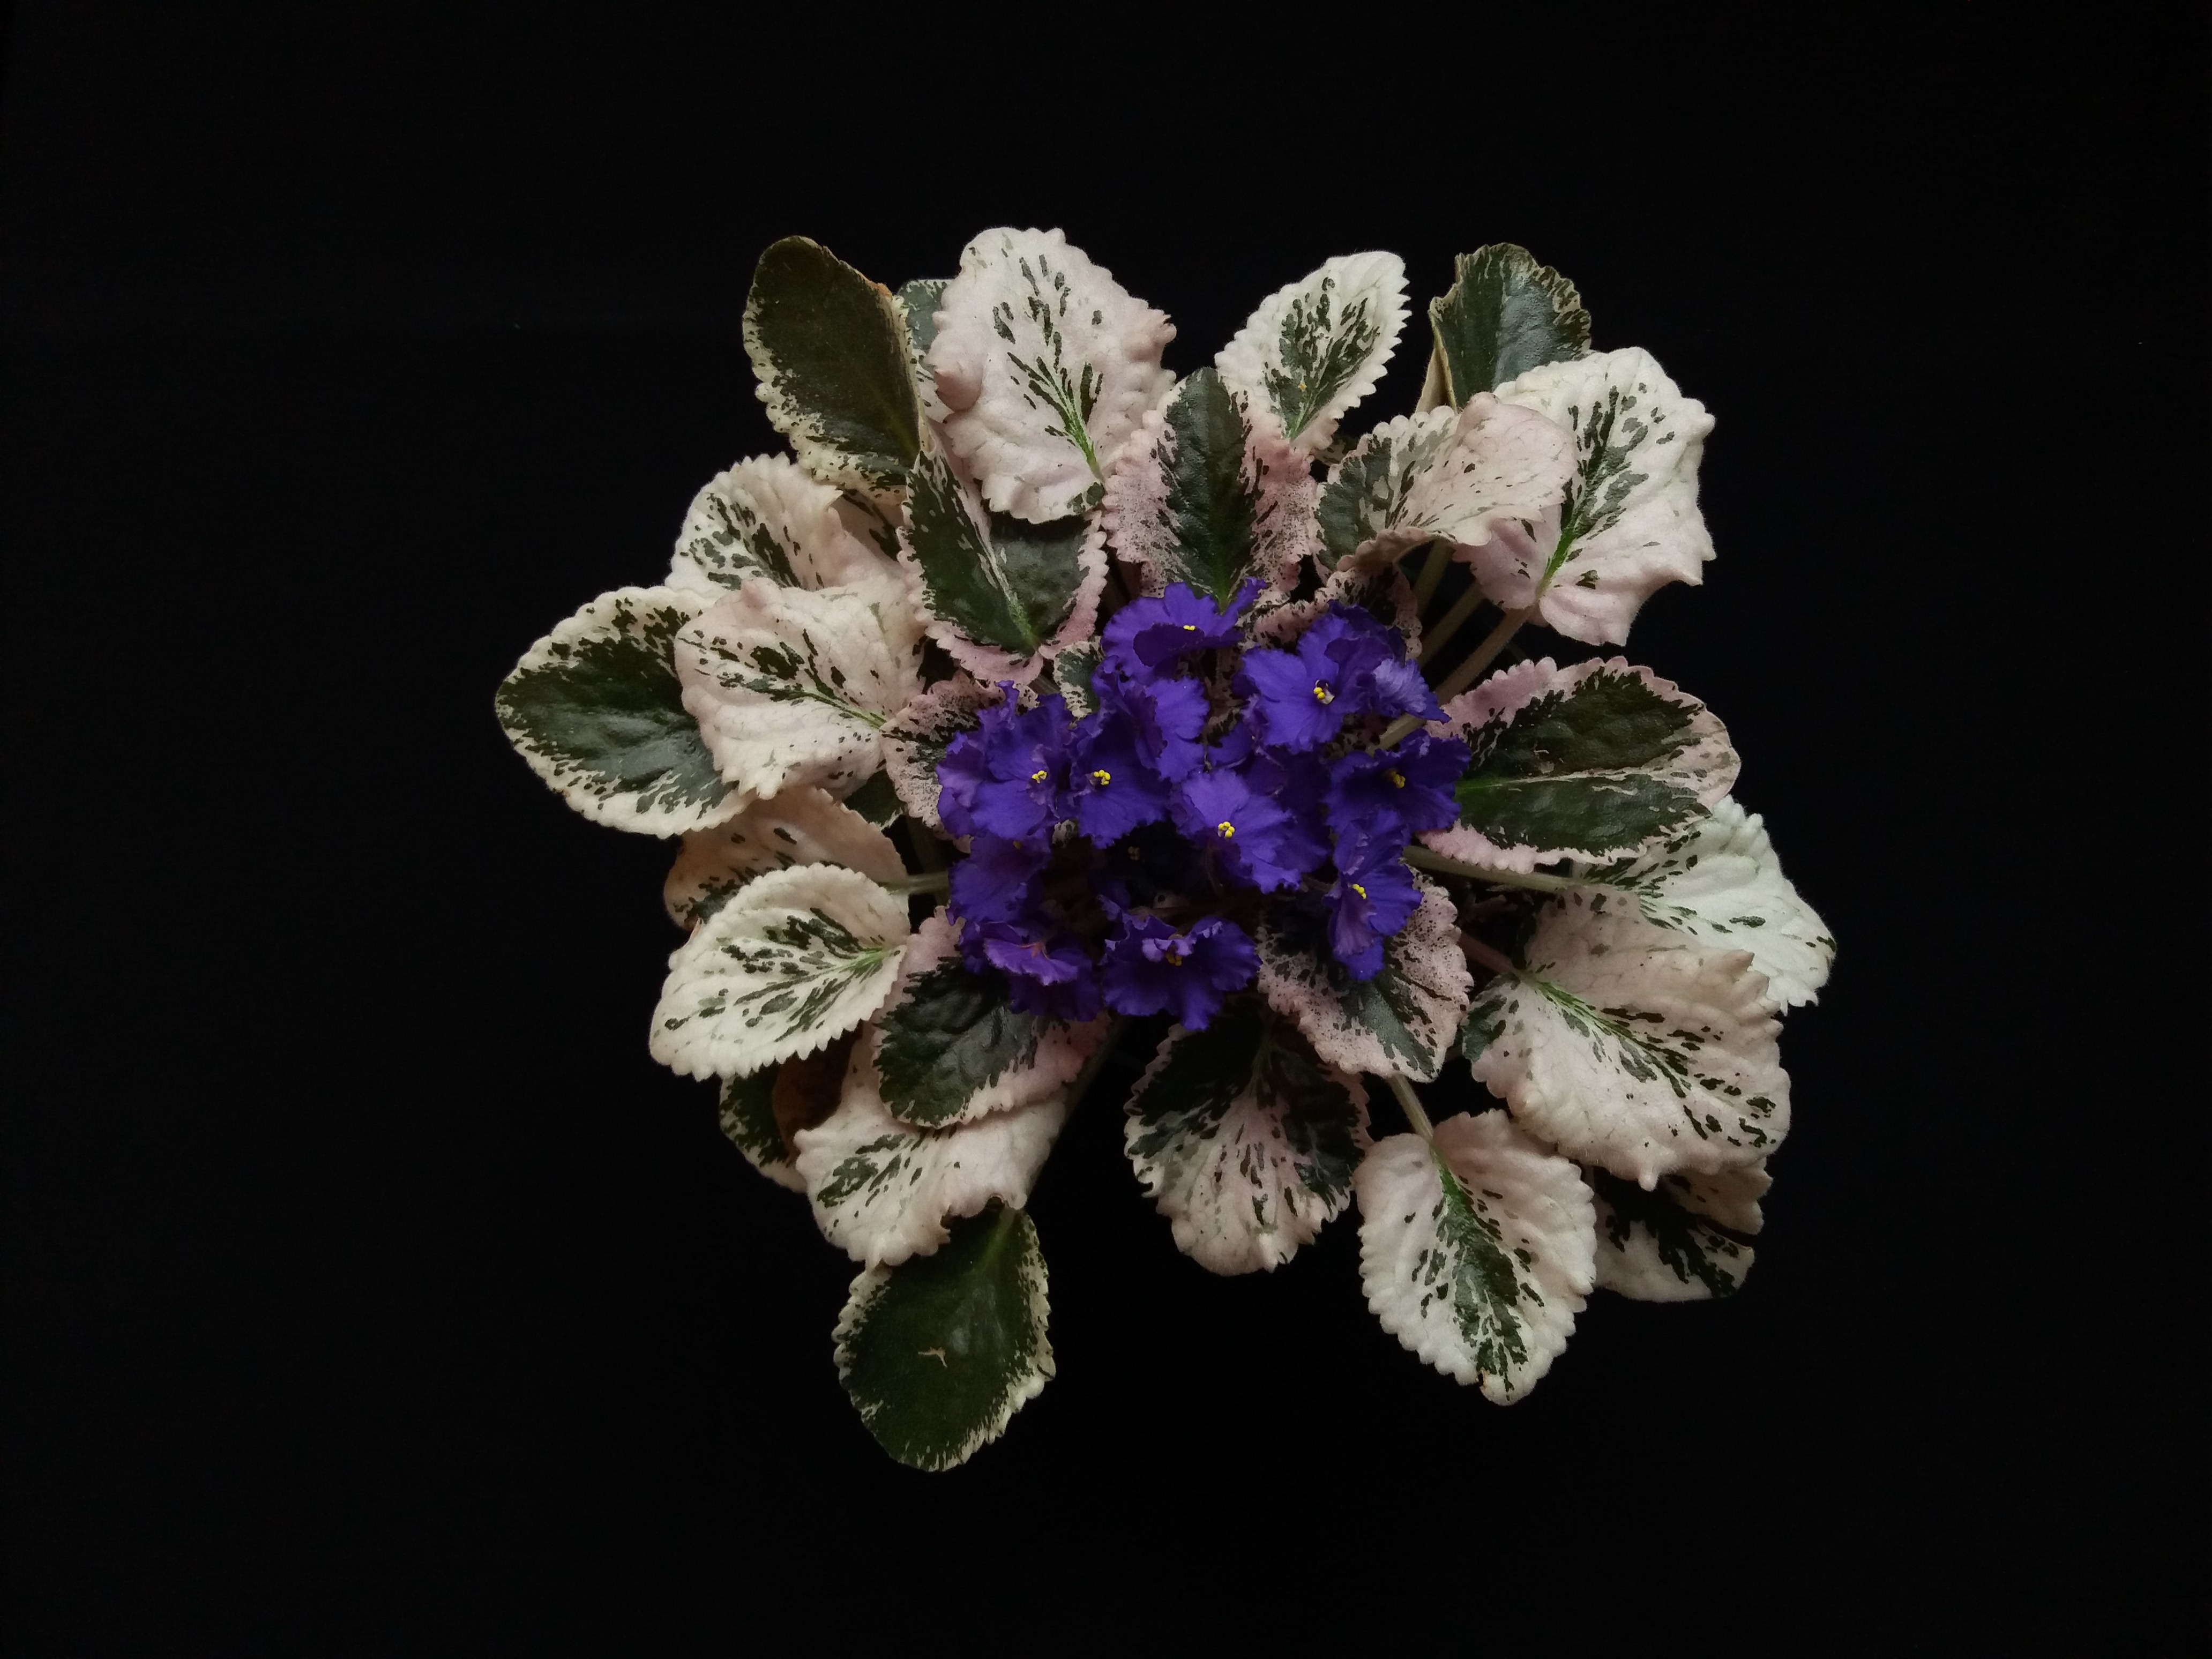
\includegraphics[width=0.68\linewidth]{../images/saintpaulia_ionantha_variegata} 

}

\caption{Variegated \textit{Saintpaulia ionantha} plant}\label{fig:variegated-saintpaulia}
\end{figure}

\end{columns}

\end{frame}

\begin{frame}{Genetics of variegation}
\protect\hypertarget{genetics-of-variegation}{}

\begin{itemize}
\tightlist
\item
  Geneticist Hermann Muller discovered an interesting genetic phenomenon
  while studying Drosophila: chromosomal neighborhoods exist that can
  silence genes that are experimentally ``relocated'' to adjacent
  regions of the chromosome.
\item
  Flies were irradiated with X rays to induce mutations in their germ
  cells.
\item
  The progeny of the irradiated flies were screened for unusual
  phenotypes. A mutation in the \emph{white} gene, near the tip of the X
  chromosome, will result in progeny with white eyes instead of the
  wild-type red color.
\item
  Some of the progeny had very unusual eyes with patches of white and
  red color.
\item
  Cytological examination revealed a chromosomal rearrangement in the
  mutant flies: present in the X chromosome was an inversion of a piece
  of the chromosome carrying the \emph{white} gene.
\item
  The white gene, which is normally located in a euchromatic region of
  the X chromosome, now finds itself near the heterochromatic
  centromere. In some cells, the heterochromatin can ``spread'' to the
  neighboring euchromatin and silence the white gene.
\end{itemize}

\end{frame}

\begin{frame}{}
\protect\hypertarget{section}{}

\begin{figure}
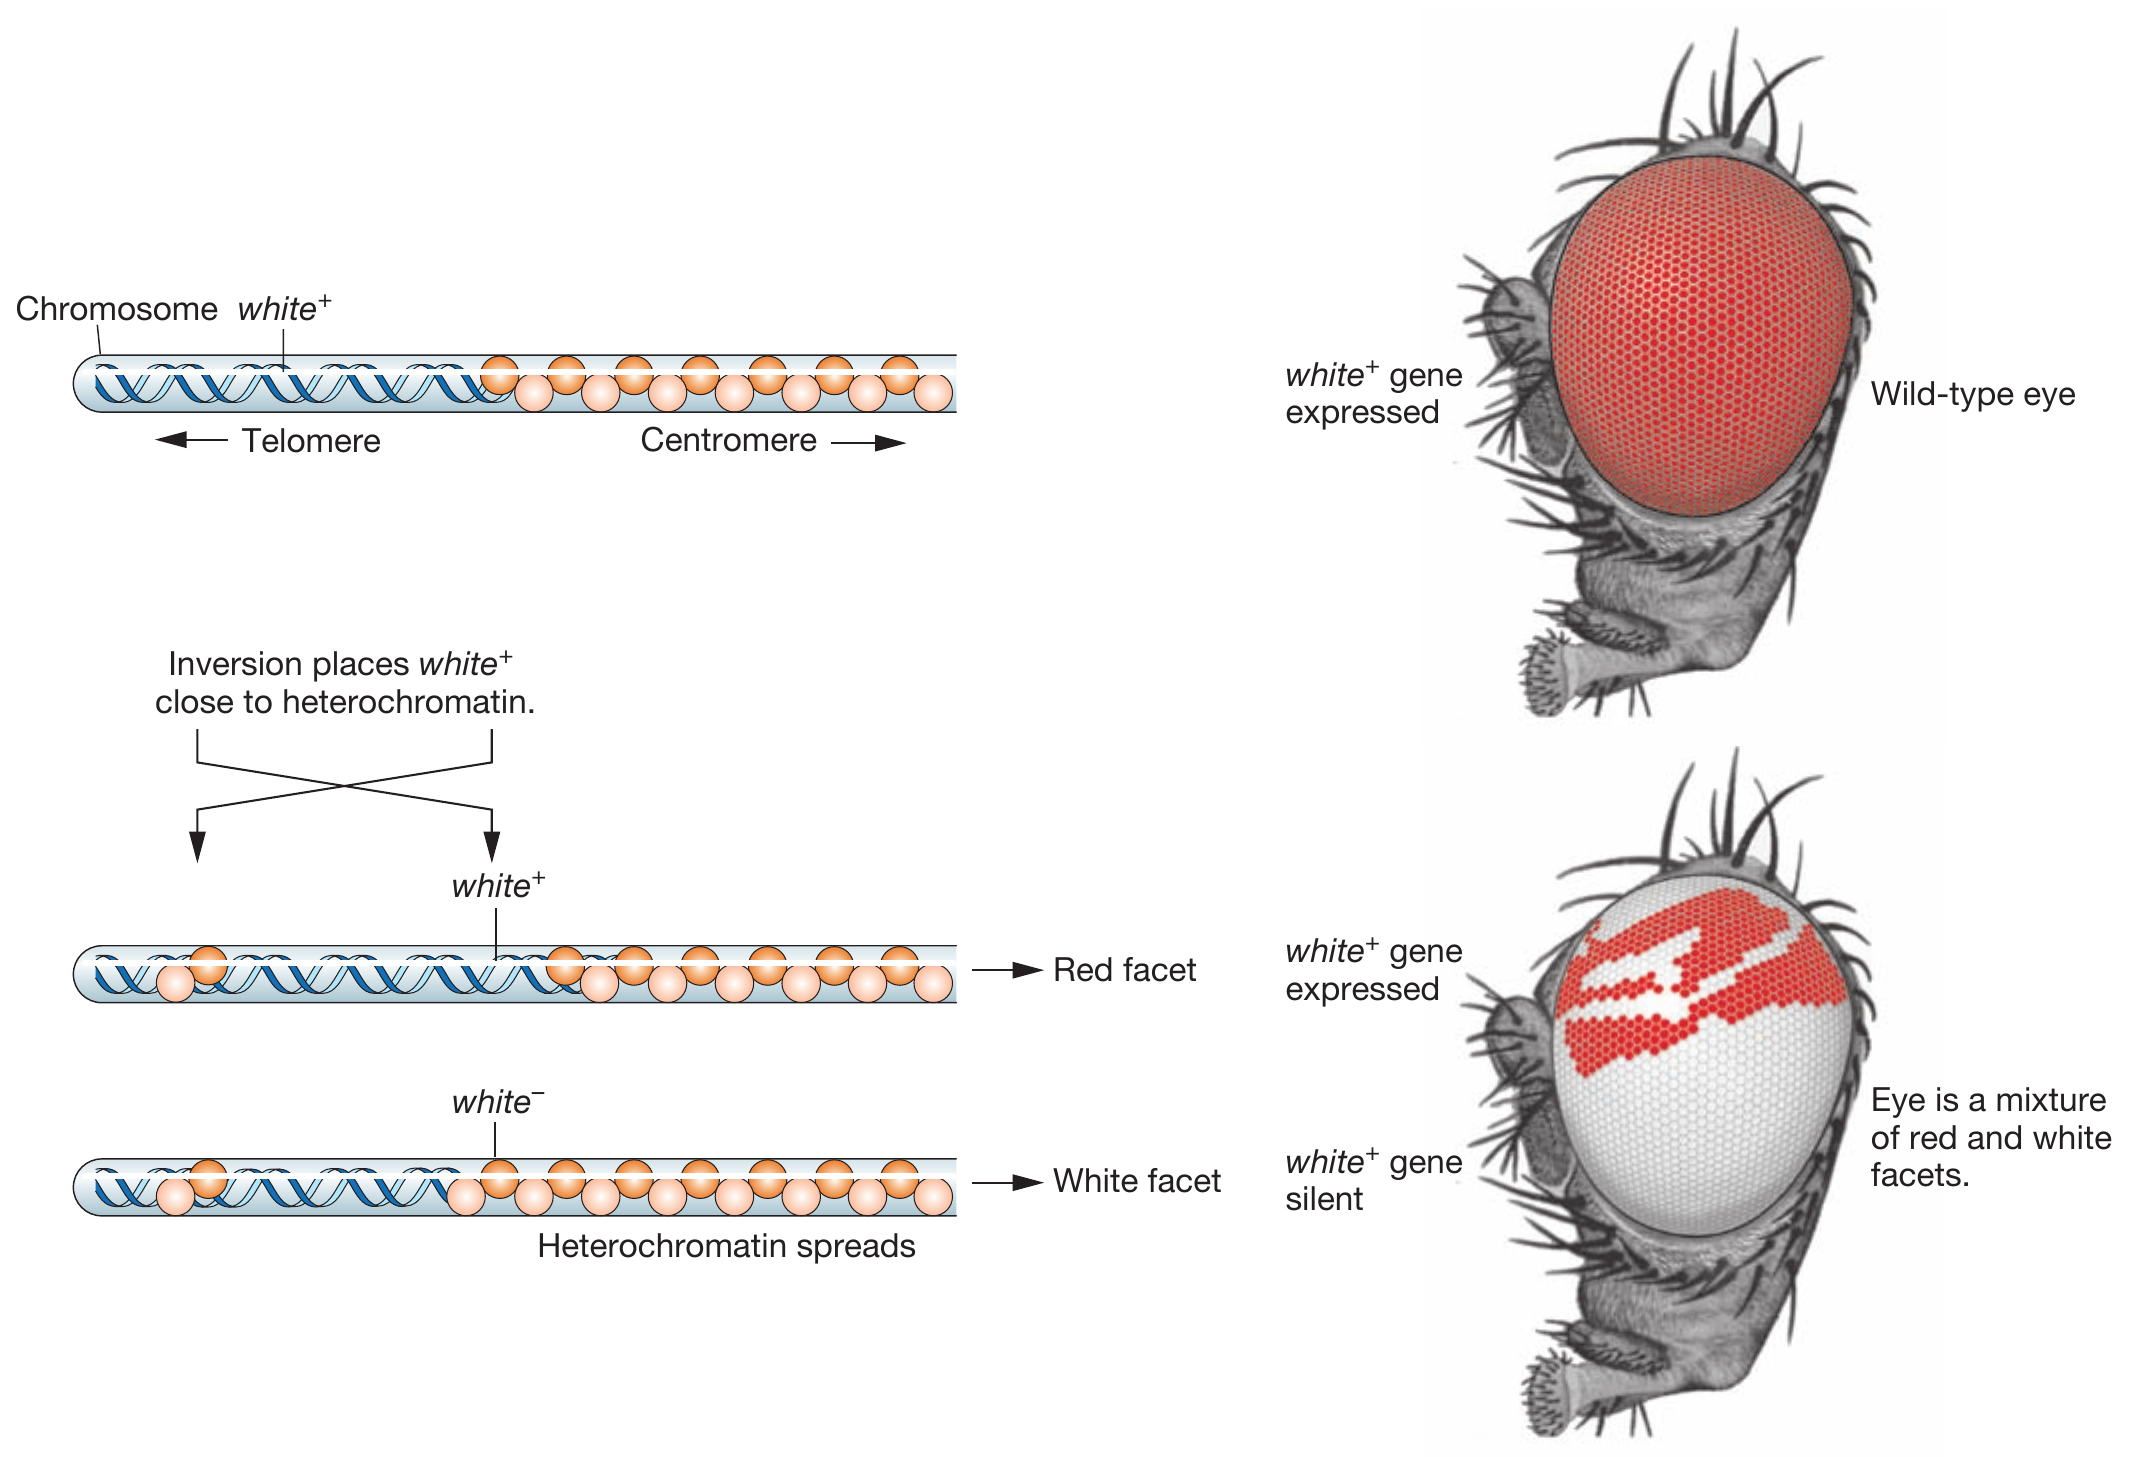
\includegraphics[width=0.55\linewidth]{./../images/drosophila_chromosomal_rearrangement_pev} \caption{Chromosomal rearrangement produces position-effect variegation. Chromosomal inversion places the wild-type white allele close to heterochromatin. The spread of heterochromatin silences the allele. Eye facets are white instead of the wild-type red wherever the allele has been silenced.}\label{fig:chromosomal-rearrangement-pev}
\end{figure}

\end{frame}

\begin{frame}{}
\protect\hypertarget{section-1}{}

\begin{itemize}
\tightlist
\item
  Patches of white tissue in the eye are derived from the descendants of
  a single cell in which the white gene has been silenced and remains
  silenced through future cell divisions.
\item
  The red patches arise from cells in which heterochromatin has not
  spread to the \emph{white} gene, and so this gene remains active in
  all its descendants.
\item
  Findings from subsequent studies in Drosophila and yeast demonstrated
  that many active genes are silenced in this mosaic fashion when they
  are relocated to neighborhoods (near centromeres or telomeres) that
  are heterochromatic.
\item
  The ability of heterochromatin to spread into euchromatin and silence
  genes is a feature common to many organisms.
\item
  This phenomenon has been called position-effect \textbf{variegation}
  (PEV).
\end{itemize}

\end{frame}

\hypertarget{development-and-pattern}{%
\section{Development and pattern}\label{development-and-pattern}}

\begin{frame}{Development}
\protect\hypertarget{development}{}

\begin{itemize}
\tightlist
\item
  Development refers to formation of different types of
  tissues/organs/cells.
\item
  Development involves production of proteins that generate specific
  structural and functional phenotypes.
\item
  From the genetic perspective, following key questions arise concerning
  number, identity, and function of genes taking part in development:

  \begin{enumerate}
  \tightlist
  \item
    Which genes are important in development?
  \item
    Where in the developing animal and at what times are these genes
    active?
  \item
    How is the expression of developmental genes regulated?
  \item
    Through what molecular mechanisms do gene products affect
    development?
  \end{enumerate}
\end{itemize}

\end{frame}

\begin{frame}{}
\protect\hypertarget{section-2}{}

\begin{itemize}
\tightlist
\item
  One of the first considerations in study of animal genetics is to go
  with certain type of organism -- Model organism. (Because it acts as
  the genetic model in animal development.)
\item
  Many genes are housekeeping genes (cellular metabolism, biosynthesis
  of macromolecules).
\item
  Some genes carry specialized taks of various organ systems, tissues
  and cells (such as antibody proteins, oxygen transporter proteins,
  etc.).
\item
  Other genes perform building of organs and tissues and the
  specification of cell types
\end{itemize}

\end{frame}

\begin{frame}{Differentiation}
\protect\hypertarget{differentiation}{}

\begin{itemize}
\tightlist
\item
  Differentiation refers to a permanent or irreversible change in the
  function of cells (relative to the single-celled zygote), which is
  often accompanied by change in their structures.
\item
  Weismann and Roux proposed that different cell types differed in their
  gene content and that each cell type contains only those genes that
  are needed for its function. But cells do not appear to lose any
  genetic material during differentiation, except in a few notable
  cases. RBC extrude their nuclei during the last stages of
  differentiation, and lymphocytes lose, during differentiation, those
  segments of antibody genes, which are not needed in a particular cell
  type.
\item
  In any differentiated cell type, only a small proportion (less than
  10\%) of the genome is transcribed to yield mRNA, e.g., 2-5 percent in
  mice liver cells, 8\% in brain cells of the toad \emph{Xenopus}, only
  1\% in \emph{Xenopus} oocyte, etc.
\end{itemize}

\end{frame}

\begin{frame}{}
\protect\hypertarget{section-3}{}

\begin{itemize}
\tightlist
\item
  In different cell types, different sets of genes are transcribed. The
  RNA sequences present in different cell types may differ from each
  other by 10-100\%. For example, the mRNAs from \emph{Xenopus laevis}
  oocytes and blastula (a stage in embryo development) embryos are
  entirely different; those from mouse liver, spleen and kidney cells
  differ from each other in sequence composition from about 15-70\%,
  etc.
\end{itemize}

\end{frame}

\begin{frame}{Embryo studies in \emph{Drosophila}}
\protect\hypertarget{embryo-studies-in-drosophila}{}

\begin{itemize}
\tightlist
\item
  Provided an understanding of formation of basic animal body plan.
\item
  Larval exoskeleton of Drosophila easily shows abnormality in the body
  plan of a mutant due to its noncellular structure.
\item
  Exoskeleton is made up of polysaccharide polymer from epidermal cells
  of embryo.
\item
  With intricate pattern of hairs, indentations, and other structures,
  the exoskeleton provides numerous landmarks to serve as indicators of
  the fates assigned to the many epidermal cells.
\item
  There are many distinct anatomical structures along the
  antero-posterior (A--P) and dorsoventral (D--V) axes.
\end{itemize}

\end{frame}

\begin{frame}{}
\protect\hypertarget{section-4}{}

\begin{itemize}
\tightlist
\item
  Effects of major mutations in either of the axes \textbf{does not}
  alter embryogenesis in very early young larva.
\item
  Recovery of exoskeleton of such stages mirrors fate of epidermal
  cells.
\item
  Only small population of cells set aside during embryogeneis
  proliferate during three larval stages (instars) and differentiate in
  the pupal stage into adult structures.
\item
  Such cells include \emph{imaginal disks}, and are easy to remove for
  expression analysis.
\end{itemize}

\end{frame}

\begin{frame}{}
\protect\hypertarget{section-5}{}

\begin{itemize}
\tightlist
\item
  Genes contributing to body plan can be cloned and characterized at
  molecular level easily
\item
  Translation products (protein) can be inferred by identifying close
  relatives in amino acid sequence.
\item
  Spatial and temporal patterns of expressions can be investigated by
  expression analysis of:

  \begin{itemize}
  \tightlist
  \item
    An mRNA, by using histochemically tagged single-stranded DNA
    sequences complementary to the mRNA to perform RNA in situ
    hybridization.
  \item
    A protein, by using histochemically tagged antibodies that bind
    specifically to that protein.
  \end{itemize}
\end{itemize}

\end{frame}

\begin{frame}{}
\protect\hypertarget{section-6}{}

\begin{figure}
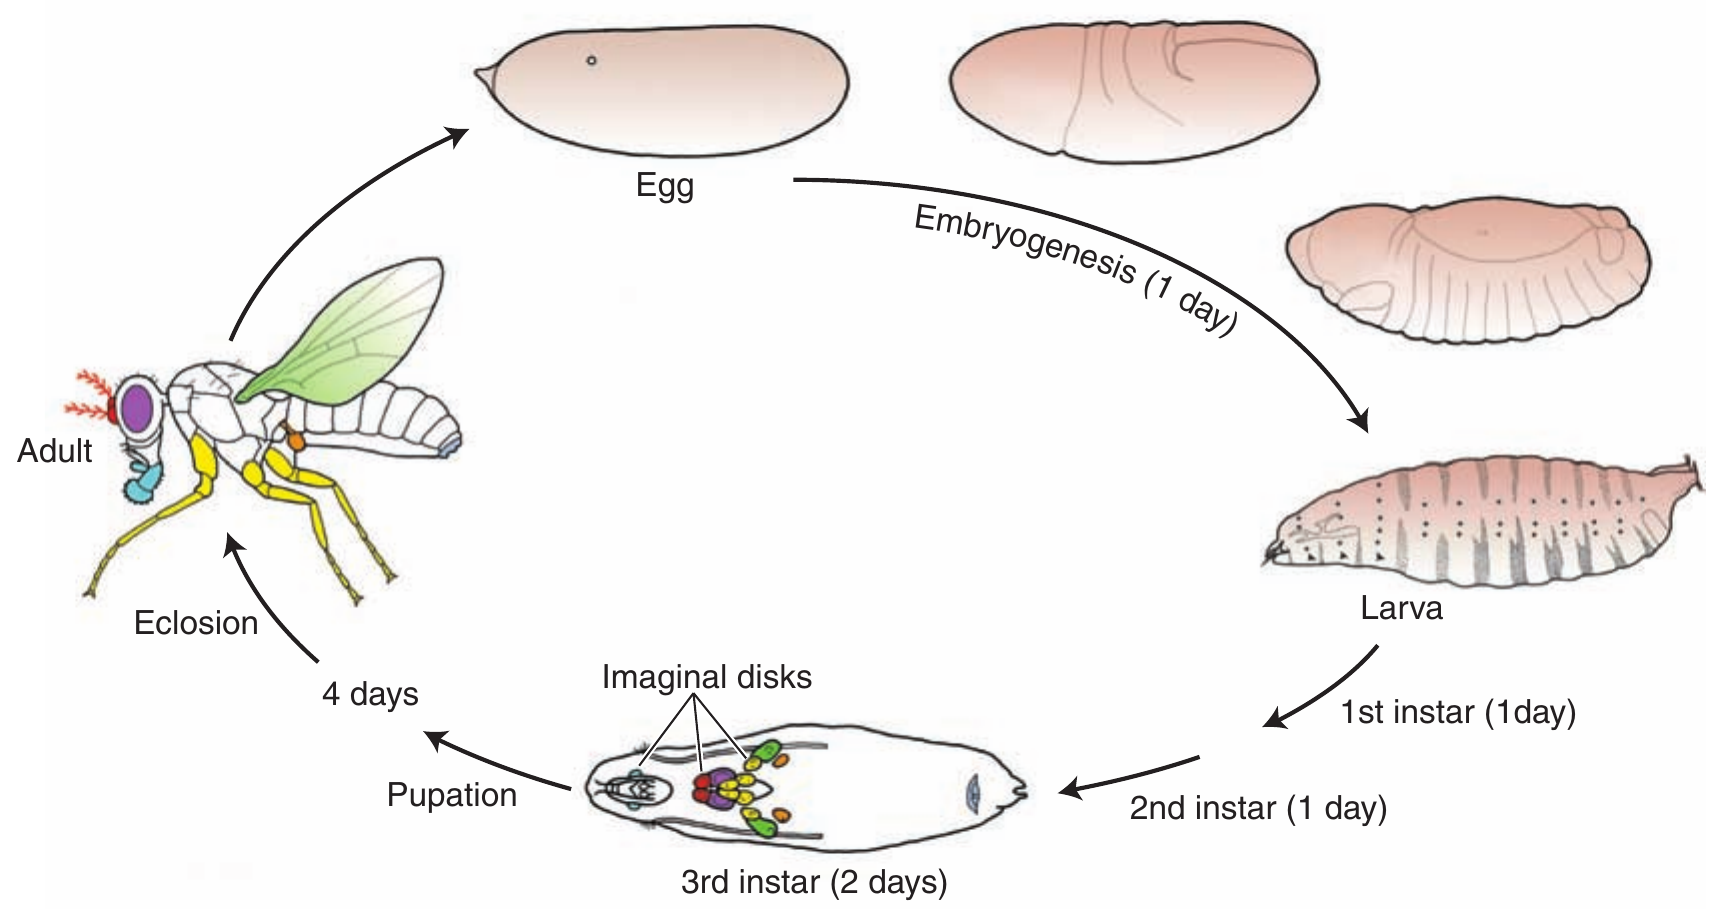
\includegraphics[width=0.55\linewidth]{./../images/drosophila_development} \caption{The larva forms in 1 day and then undergoes several stages of growth during which the imaginal disks and other precursors of adult structures proliferate. These structures differentiate during pupation, and the adult fly hatches (eclosion) and begins the cycle again.}\label{fig:drosophila-development}
\end{figure}

\end{frame}

\begin{frame}{Extrapolating information}
\protect\hypertarget{extrapolating-information}{}

\begin{itemize}
\tightlist
\item
  There are numerous homeobox genes within \emph{Drosophila} genome.
\item
  Homeotic gene detection depends on DNA base-pair complementarity.
\item
  Hybridization experiments can be done with \emph{moderate stringency
  conditions}.
\item
  Homeobox genes have been searched for in other animals, by means of
  \emph{zoo blots} by using radioactive Drosophila homeobox DNA as the
  probe.
\item
  This approach led to the discovery of homologous homeobox sequences in
  many different animals, including humans and mice.
\item
  Homeotic mutants have following features:

  \begin{itemize}
  \tightlist
  \item
    Developmental pathways are changed dramatically due to single
    homeotic gene mutation
  \item
    Structure formed in mutant is alike to well-developed another body
    part
  \item
    Transform the identity of serially reiterated structures
  \end{itemize}
\item
  Systematic searches for homeotic genes have led to the identification
  of eight loci, now referred to as Hox genes, that affect the identity
  of segments and their associated appendages in Drosophila.
\end{itemize}

\end{frame}

\begin{frame}{}
\protect\hypertarget{section-7}{}

\begin{figure}
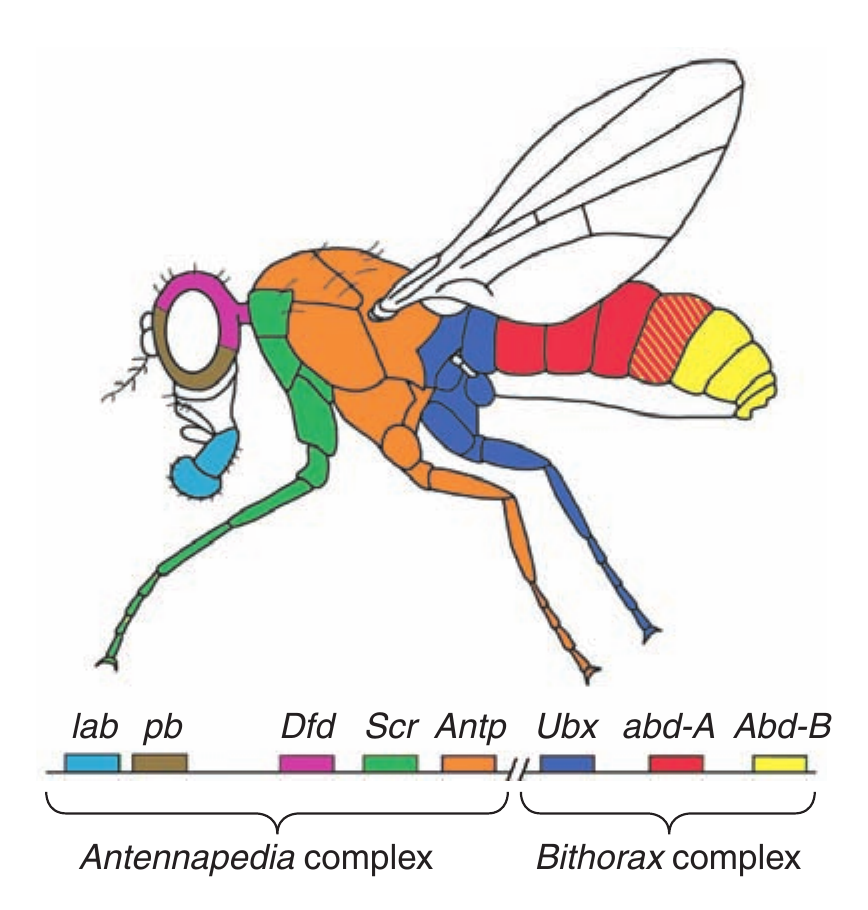
\includegraphics[width=0.35\linewidth]{./../images/drosophila_hox_genes} \caption{The Hox genes of Drosophila. Eight Hox genes regulate the identity of regions within the adult. The color coding identifies the segments and structures that are affected by mutations in the various Hox genes.}\label{fig:drosophila-hox-genes}
\end{figure}

\end{frame}

\begin{frame}{Summary}
\protect\hypertarget{summary}{}

\begin{itemize}
\tightlist
\item
  Despite vast differences in appearance and anatomy, animals have in
  common a toolkit of genes that govern development.
\item
  Distinguishing feature of toolkit genes is the typical presence of
  numerous independent cisacting regulatory elements that govern gene
  expression in different spatial domains and at different stages of
  development.
\item
  This toolkit is a small fraction of all genes in the genome, and most
  of these toolkit genes control transcription factors and components of
  signal-transduction pathways.
\item
  Individual toolkit genes typically have multiple functions and affect
  the development of different structures at different stages.
\item
  The development of the growing embryo and its body parts takes place
  in a spatially and temporally ordered progression.
\end{itemize}

\end{frame}

\begin{frame}{}
\protect\hypertarget{section-8}{}

\begin{itemize}
\tightlist
\item
  Spatially restricted patterns of gene expression are products of
  combinatorial regulation. Each pattern of gene expression has a
  preceding causal basis. New patterns are generated by the combined
  inputs of preceding patterns.
\item
  As an example, the positioning of pair-rule stripes and the
  restriction of appendage-regulatory-gene expression to individual
  segments requires the integration of numerous positive and negative
  regulatory inputs by cis-acting regulatory elements.
\item
  Post-transcriptional regulation at the RNA level adds another layer of
  specificity to the control of gene expression.
\item
  Alternative RNA splicing and translational control by proteins and
  miRNAs also contribute to the spatial and temporal control of
  toolkit-gene expression.
\item
  Combinatorial control is key to both the \textbf{specificity} and the
  \textbf{diversity} of gene expression and toolkit-gene function.
\item
  The modularity of cis-acting regulatory elements allows for
  independent spatial and temporal control of toolkit-gene expression
  and function. They act as switches in the developmental control of
  gene expression.
\end{itemize}

\end{frame}

\hypertarget{genetics-of-cancer}{%
\section{Genetics of cancer}\label{genetics-of-cancer}}

\begin{frame}{}
\protect\hypertarget{section-9}{}

\begin{itemize}
\tightlist
\item
  Somatic cells of higher eukaryotes have limited life span, and their
  growth and divisions are highly regulated.
\item
  But occasionally, some cells show uncontrolled division and growth,
  and an ability to grow in inappropriate locations; these cells are
  said to be cancerous or tumorigenic and they produce cancer.
\item
  Uncontrolled growth in non-circulatory tissues produces solid tumors.
\item
  A malignant tumor, or \textbf{cancer}, is an aggregate of cells, all
  descended from an initial aberrant founder cell.
\item
  When tumor becomes \textbf{malignant} or \textbf{cancerous}, its cells
  detach and migrate to other parts of body where they produce secondary
  tumors; this phenomenon is called \textbf{metastasis}.
\item
  \textbf{Benign} or noncancerous tumors do not exhibit metastasis.
\end{itemize}

\end{frame}

\begin{frame}{}
\protect\hypertarget{section-10}{}

\begin{itemize}
\tightlist
\item
  Cancerous cells are produced due to the following three types of
  changes:

  \begin{itemize}
  \tightlist
  \item
    Immortalization,
  \item
    Transformation
  \item
    Metastasis.
  \end{itemize}
\item
  Cancer arises through:

  \begin{enumerate}
  \tightlist
  \item
    An increased mutation rate that creates genetic variation and
  \item
    Selection of cells for increased proliferation rates; several cycles
    of these events occur in the progression of cancer. (Singh 2018),
    page 386.
  \end{enumerate}
\end{itemize}

\end{frame}

\begin{frame}{}
\protect\hypertarget{section-11}{}

\begin{itemize}
\tightlist
\item
  Cancer researchers have identified genes that, when mutated, can
  contribute to the development of a cancerous state. In it, genes or
  mutant genes actively promote cell division.
\item
  The genes are called \textbf{oncogenes}, from the Greek word for
  `tumor.'
\item
  Oncogenes: Many cancers involve the overexpression of certain genes or
  the abnormal activity of their mutant protein products; They result in
  dominant mutations, usually owing to their inappropriate activation.
\item
  In contrast, tumor-suppressor genes encode proteins whose loss of
  activity can contribute to a cancerous state. As such, they are
  recessive mutations.
\item
  These genes were first discovered in the genomes of RNA viruses that
  are capable of inducing tumors in vertebrate hosts.
\item
  Later, the cellular counterparts of these viral oncogenes were
  discovered in many different organisms ranging from \emph{Drosophila}
  to humans.
\end{itemize}

\end{frame}

\begin{frame}{Tumor producing retroviruses and viral oncogenes}
\protect\hypertarget{tumor-producing-retroviruses-and-viral-oncogenes}{}

\begin{itemize}
\tightlist
\item
  Understanding of genetic basis of cancer has come from the study of
  tumor-inducing viruses.
\item
  Many of these viruses have a genome composed of RNA instead of DNA.
\item
  After entering a cell, the viral RNA is used as a template to
  synthesize complementary DNA, which is then inserted at one or more
  positions in the cell's chromosomes.
\item
  The synthesis of DNA from RNA is catalyzed by the viral enzyme reverse
  transcriptase. This reversal of the normal flow of genetic information
  from DNA to RNA has prompted biologists to call these pathogens
  \textbf{retroviruses}.
\end{itemize}

\end{frame}

\begin{frame}{}
\protect\hypertarget{section-12}{}

\begin{itemize}
\tightlist
\item
  The first tumor-inducing virus was discovered in 1910 by Peyton Rous;
  it caused a special kind of tumor, or sarcoma, in the connective
  tissue of chickens and has since been called the Rous sarcoma virus.
\item
  Rous was awarded the Nobel Prize in Physiology or Medicine for the
  significance of his discovery in 1966. Modern research has shown that
  the RNA genome of this retrovirus contains four genes: \emph{gag},
  \emph{pol}, \emph{env}
\item
  \textbf{Other examples}:

  \begin{itemize}
  \tightlist
  \item
    Breast cancer (\emph{BRCA2}): Autosomal dominant. Tumor suppressor
    defect giving predisposition to breast and other cancers
  \item
    \emph{TLF}: Colon cancer
  \item
    \emph{Gli1}: Basal-cell carcinoma
  \item
    \emph{DPC4}: Pancreatic and colon
  \item
    \emph{hNotch1}: Leukemia, lymphoma
  \end{itemize}
\end{itemize}

\end{frame}

\hypertarget{immunogenetics}{%
\section{Immunogenetics}\label{immunogenetics}}

\begin{frame}{Introduction}
\protect\hypertarget{introduction}{}

\begin{columns}[T,onlytextwidth]
  \small
  \column{.35\linewidth}
  
  \begin{itemize}
  \item The immune system keeps a repertoire of B cells that are poised to make antibodies to invading pathogens. 
  \item When one of these B-cell antibodies is needed, the B cell starts dividing so that many antibodies can be produced and they are available to attack the pathogen. 
  \item Some of these clones are refined by mutation to make a more specific antibody.
  \end{itemize}
  
  \column{0.65\linewidth}
  

\begin{center}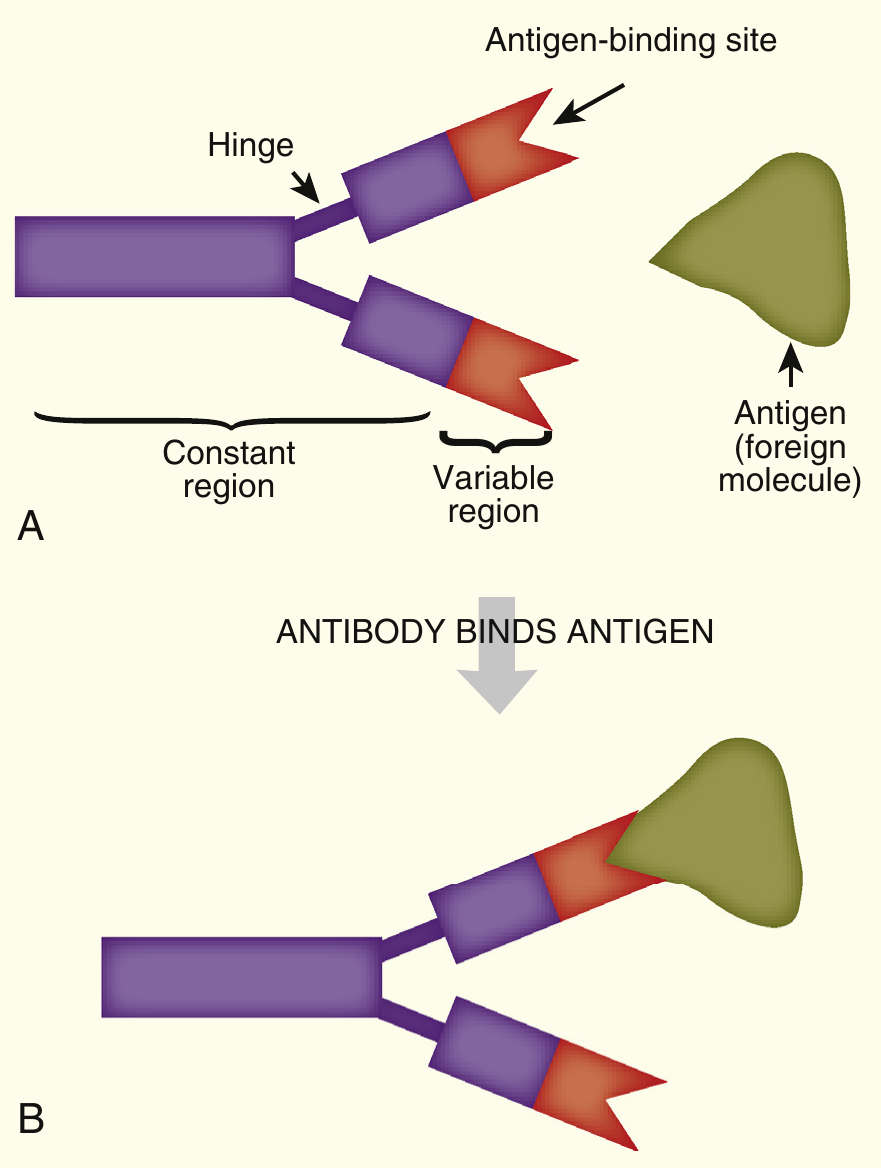
\includegraphics[width=0.5\linewidth]{./../images/antibody_antigen_recognition} \end{center}

\end{columns}

\end{frame}

\begin{frame}{}
\protect\hypertarget{section-13}{}

\begin{itemize}
\tightlist
\item
  Acquired immunity is divided into two branches. Humoral immunity is
  mediated by antibodies in blood plasma, which are produced by B cells.
  The second part is cellular immunity, which is mediated by T cells.
\item
  Antibodies recognize epitopes or specific regions of the invading
  pathogen.
\item
  Antibodies are very diverse in structure so that all the pathogens can
  be recognized.
\item
  Antibodies are produced by shuffling gene segments rather than having
  one gene code for each different antibody; the process is called
  \textbf{V(D)J} recombination.
\end{itemize}

\end{frame}

\begin{frame}{}
\protect\hypertarget{section-14}{}

\begin{itemize}
\tightlist
\item
  ELISA (diagnostics) procedure uses antibodies for clinical use.
\item
  Antibodies of various mixtures with variying affinities to antigen/s
  is reffered to as polyclonal antibody. However such antibodies are of
  little use for a specific, accurate assay.
\item
  Pure antibody made by a single line of cells is known as a
  \textbf{monoclonal antibody}.
\item
  An example of antibody generation technology is by exploiting myelomas
  (naturally occurring cancers) derived from B cells; they therefore
  express immunoglobulin genes, as long as they are given proper
  nutrients.
\item
  To make monoclonal antibodies, scientists fuse the relatively delicate
  B cell, which is making the required antibody, to a myeloma cell. The
  resulting hybrid is called a \textbf{hybridoma}.
\end{itemize}

\end{frame}

\begin{frame}{}
\protect\hypertarget{section-15}{}

\begin{figure}
\begin{columns}[T,onlytextwidth]
\column{.70\linewidth}
\begin{center}
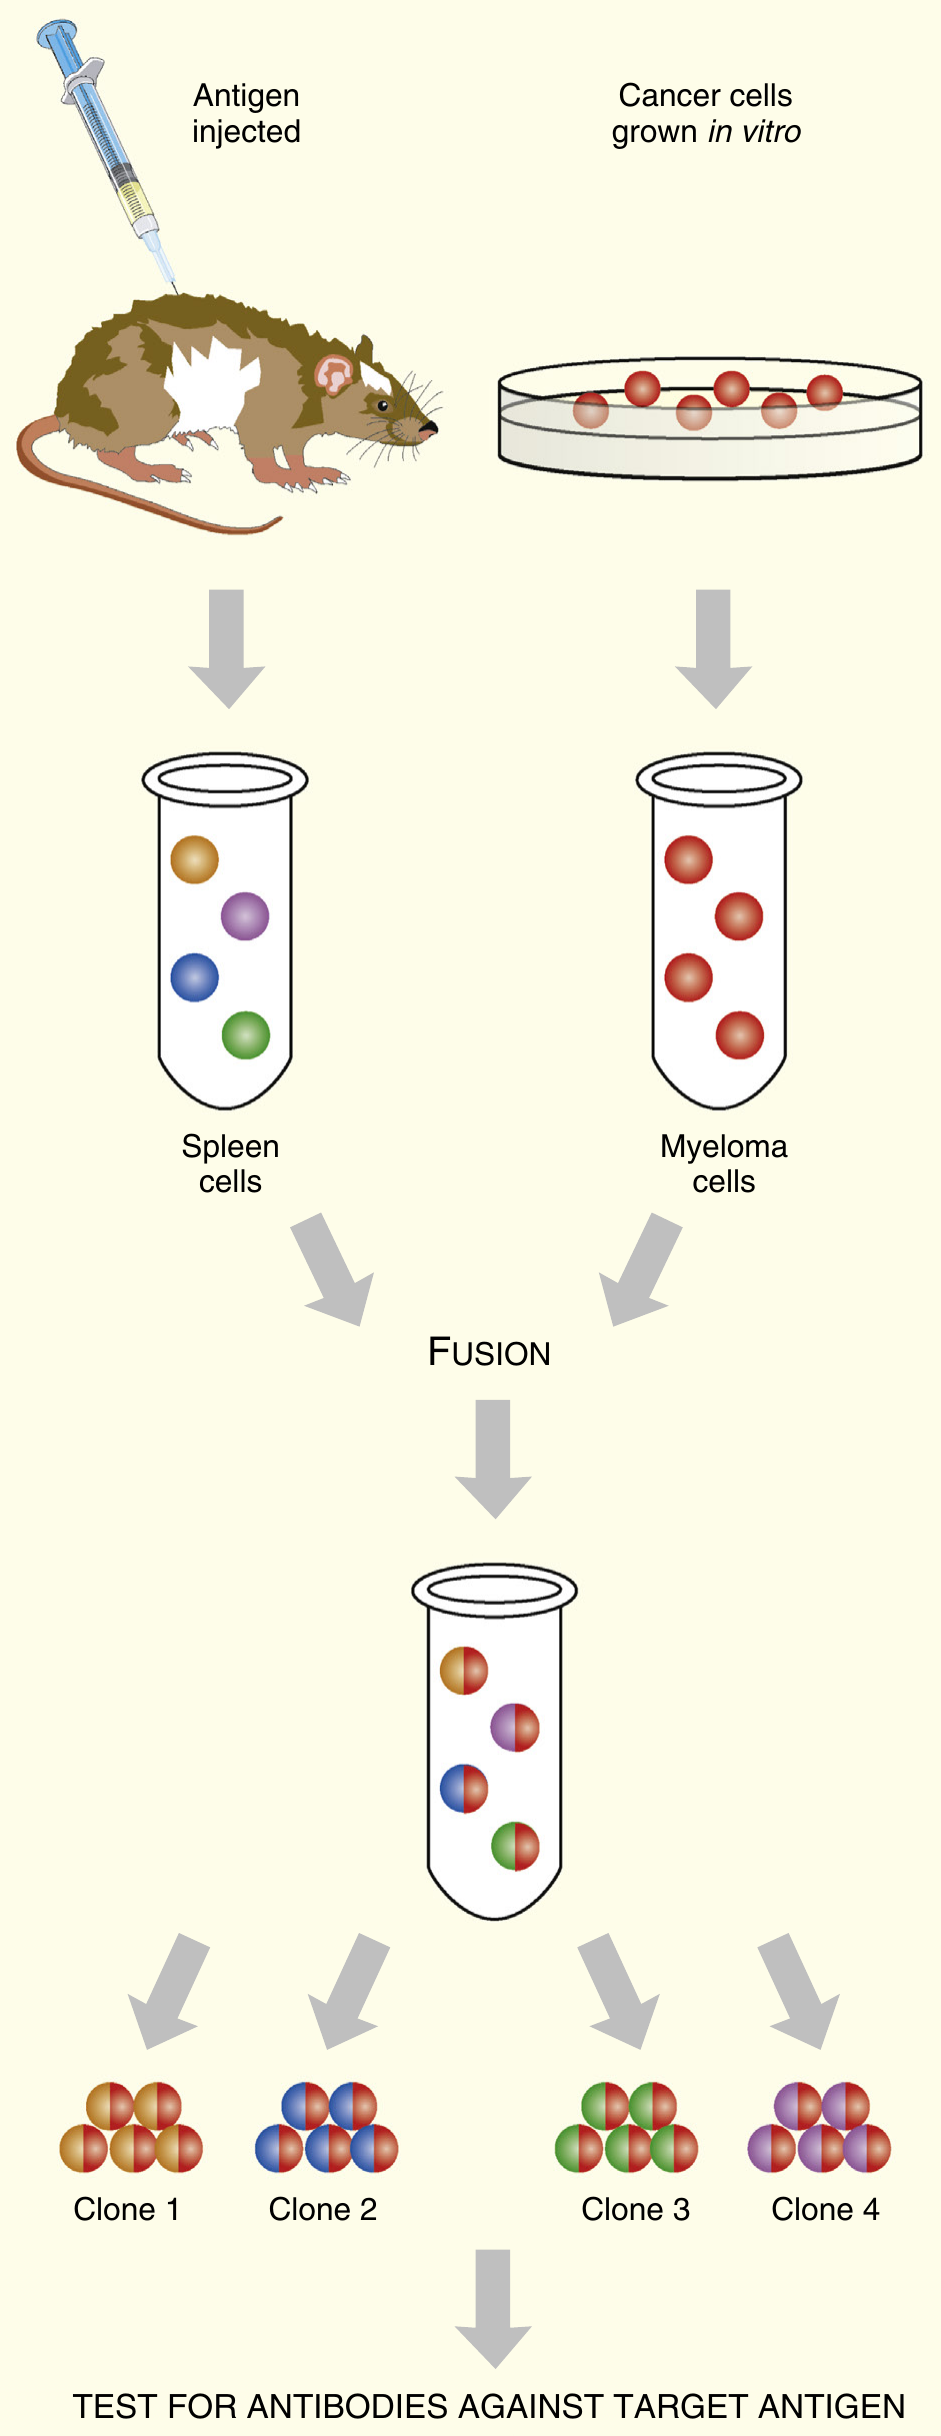
\includegraphics[width=0.28\linewidth]{./../images/hybridoma_principle.png}
\end{center}
\column{.30\linewidth}
\caption{\newline \textbf{Principle of the Hybridoma} \newline Monoclonal antibodies derive from a single antibody-producing B cell. The antigen is first injected into a mouse to provoke an immune response. The spleen is harvested because it harbors many activated B cells. The spleen cells are short-lived in culture, so they are fused to immortal myeloma cells. The hybridoma cells are cultured and isolated so each hybrid is separate from the other. Each hybrid clone can then be screened for the best antibody to the target protein.}
\label{fig:monoclonal-antibody-hybridoma}
\end{columns}
\end{figure}

\end{frame}

\begin{frame}{Vaccination}
\protect\hypertarget{vaccination}{}

\begin{itemize}
\tightlist
\item
  Vaccination takes advantage of immune memory.
\item
  Vaccines consist of various derivatives of infectious agents that no
  longer cause disease but are still antigenic; that is, they induce an
  immune response.
\item
  For example, bacteria killed by heat are sometimes used. The antigens
  on the dead bacteria stimulate B-cell division.
\item
  Some of the B cells form memory cells so, later, when living germs
  corresponding to the vaccine attack the vaccinated person, the immune
  system is prepared.
\end{itemize}

\end{frame}

\hypertarget{bibliography}{%
\section{Bibliography}\label{bibliography}}

\begin{frame}{References}
\protect\hypertarget{references}{}

\hypertarget{refs}{}
\leavevmode\hypertarget{ref-singh2018fundamentals}{}%
Singh, BD. 2018. \emph{Fundamentals of Genetics}. Kalyani Publishers.

\end{frame}




\end{document}
